%! TEX program = lualatex
\documentclass[12pt,a4paper]{article} 

% Packages for formatting
\usepackage{fontspec}
\usepackage[ngerman]{babel}
\usepackage{geometry} 
\geometry{margin=1in} 
\usepackage{setspace} 
\usepackage{hyperref} 
\usepackage{xcolor}
\usepackage{amsmath, amssymb} % for align*
\usepackage{amsthm} % neue Theorem-Umgebungen
\usepackage{enumitem} % für schöne Listen (Teilaufgaben)
\usepackage{mathbbol}
\usepackage{graphicx}
\usepackage{amssymb}
\usepackage{gensymb}
\usepackage{stackengine}

\DeclareMathAlphabet\mathbb{U}{fplmbb}{m}{n}
% Style settings
\pagecolor{darkgray}      % sets background color to black 
\color{gray}          % sets text color to white

% Change subsection to use a, b, c instead of 1, 2, 3
\renewcommand{\thesubsection}{\alph{subsection})}
\newcommand{\zz}{\stackinset{c}{2.5pt}{c}{-2.5pt}{\textsf{Z}}{\textsf{Z}}}
% Title page info 
\title{Blatt 09}
\author{Hannes Rall \\ Albert-Ludwigs-University}
\date{\today}

\begin{document}
% Title page 
\begin{titlepage}
    \centering
    \vspace*{2cm}
    {\Huge\itshape Blatt 09\par}
    \vspace{2cm}
    {\Large\textsc{Hannes Rall}\par}
    \vfill
    {\large Albert-Ludwigs-University\\}
    \vspace{1cm}
    {\large\today\par}
\end{titlepage}

\newpage
\section*{Aufgabe 25}
Sei $ABC$ ein sphärisches Dreieck und sei $A_pB_pC_p$ das Polardreieck zu $ABC$.\\
$\zz$ : Dann ist $ABC$ das Polardreieck zu $A_pB_pC_p$.
\begin{proof}
Da $A_pB_pC_p$ das Polardreieck zu $ABC$ ist, gilt mit $\epsilon = sign(\det(A,B,C))$:

 \begin{alignat*}{3}     
 A_p &= \epsilon \frac{B \times C}{|B \times C|} \qquad 
     &B_p &= \epsilon \frac{C \times A}{|C \times A|} \qquad     
     &C_p &= \epsilon \frac{A \times B}{|A \times B|} \end{alignat*}
Nun berechnen wir $\epsilon_p$: \\
\begin{align*}
    \epsilon_p &= sign(\det(A_p, B_p, C_p)) \\
               &= sign \left(\det \left(\epsilon \frac{B \times C}{|B \times C|}, \epsilon \frac{C \times A}{|C \times A|}, \epsilon \frac{A \times B}{|A \times B|} \right)\right) \\
               &= sign \left(\frac{\epsilon^{3}}{|B \times C||C \times A||A \times B|} \det (B \times C, C \times A, A \times B)\right) \\
               &= sign \left(\frac{\epsilon^{3}}{|B \times C||C \times A||A \times B|} \cdot (-1)(-1) \cdot \det (A \times B, B \times C, C \times A)\right) \\
               &= sign \left( \frac{\epsilon}{|B \times C||C \times A||A \times B|} \cdot \det(A, B, C)^2 \right) \\
               &= sign \left( \epsilon \frac{\det(A, B, C)^2}{|B \times C||C \times A||A \times B|} \right) \\
               &= \epsilon
\end{align*}
Wir verwenden Rechenregeln für die Determinante und * aus Bemerkung IV.2.11. Der letzte Schritt folgt, da der Bruch auf jeden Fall positiv ist, aufgrund des Quadrates und der Norm. \\
\\
Jetzt schauen wir uns $C''$ an und verwenden, dass das Kreuzprodukt eine Bilinearform ist und Rechenregeln für das Kreuzprodukt sowie für die Determinante:
\begin{align*}
C'' &= \epsilon_p \frac{A_p \times B_p}{|A_p \times B_p|} = \epsilon \frac{\epsilon \frac{B \times C}{|B \times C|} \times \epsilon \frac{C \times A}{|C \times A|} }{|\epsilon \frac{B \times C}{|B \times C|}  \times \epsilon \frac{C \times A}{|C \times A|}|} = \epsilon \frac{\frac{\epsilon^2}{|B \times C||C \times A|} (B \times C) \times (C\times A)}{\left|\frac{\epsilon^2}{|B \times C||C \times A|} (B \times C) \times (C\times A) \right|} \\
    &= \epsilon \frac{\frac{\epsilon^2}{|B \times C||C \times A|} (B \times C) \times (C\times A)}{\left|\frac{\epsilon^2}{|B \times C||C \times A|} \right| \left|(B \times C) \times (C\times A) \right|} =  \epsilon \frac{\frac{\epsilon^2}{|B \times C||C \times A|} (B \times C) \times (C\times A)}{\frac{\epsilon^2}{|B \times C||C \times A|} \left|(B \times C) \times (C\times A) \right|} \\
    &= \epsilon \frac{(B \times C) \times(C \times A)}{|(B \times C) \times(C \times A)|} = \epsilon \frac{C \det(B, C, A)}{|C \det(B, C, A)|} = \epsilon \frac{C \det(B, C, A)}{|C||\det(B, C, A)|} = C \cdot \frac{\epsilon \det (A, B, C)}{|\det(A, B, C)|}
\end{align*}
\newpage
\noindent 1. Fall: $\det(A, B, C) > 0$, dann ist $\epsilon = 1$ und es folgt:
\begin{align*}
    C \cdot \frac{\epsilon \det(A, B, C)}{|\det(A, B, C)|} = C \cdot \frac{\det(A, B, C)}{\det(A, B, C)} = C
\end{align*}
2. Fall: $\det(A, B, C) < 0$, dann ist $\epsilon = -1$ und es folgt:
\begin{align*}
C \cdot \frac{\epsilon \det(A, B, C)}{|\det(A, B, C)|} = C \cdot \frac{-\det(A, B, C)}{-\det(A, B, C)} = C
\end{align*}
\noindent Also folgt insgesamt $C'' = C$. Analog folgen $A'' = A$ und $B'' = B$. \\
Somit ist $ABC$ das Polardreieck von $A_pB_pC_p$.
\end{proof}

\newpage
\section*{Aufgabe 27}
\subsection*{(i) Bearbeiten Sie alle Aufgaben und Fragen des Schülerarbeitsblattes.}
\begin{figure}[htbp]     
    \centering             
    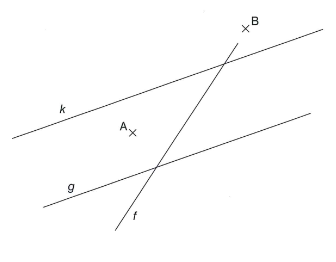
\includegraphics[width=0.8\textwidth]{Euklidische_Ebene.png}     
    \caption{24}     
    \label{fig:24} 
\end{figure}
\subsubsection*{Überprüfe, ob in den folgenden Beispielen Inzidenz vorliegt:}
\noindent Liegt der Punkt A auf der Geraden g?\\ 
Nein. \\
Schneidet die Gerade g die Gerade f?\\
Ja. \\
Schneidet die Gerade g die Gerade k?\\ 
Nein bzw kann man nicht sagen, falls sie sehr sehr leicht geneigt sind. \\
Liegt der Punkt B auf der Geraden f?\\ 
Ja sieht so aus. Wenn nicht ist es ein Militmeter und die Zeichnung irreführend.\\

\newpage
\begin{figure}[htbp]     
    \centering             
    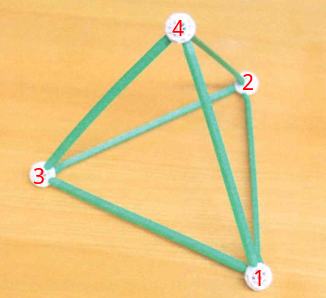
\includegraphics[width=0.8\textwidth]{Tetraeder.png}     
    \caption{24}     
    \label{fig:24} 
\end{figure}
\subsubsection*{Überprüfe ob die drei genannten Axiome erfüllt sind.}
1) Jeder Gerade enthält mindestens zwei Punkte.\\
Ja und zwar die jeweiligen Eckpunkte.\\
2) Zu zwei verschiedenen Punkten gibt es stets genau eine Gerade, auf der die beiden Punkte liegen.\\
Ja und zwar die jeweilige Kante die die Eckpunkte verbindet.\\
3) Es gibt mindestens drei Punkte, die nicht alle auf derselben Geraden liegen.\\
Ja denn es gibt 4 Punkte, also mindestens 3 und zb die unteren drei liegen nicht alle auf derselben Geraden.\\
\subsubsection*{Überprüfe ob das Prallelenaxoim in der Tetraeder-Geometrie erfüllt ist.}
O.B.d.A ist zur Geraden durch 1 und 2 nur die Gerade durch 3 und 4 parallel. Also ja das Axiom gilt.

\newpage
\begin{figure}[htbp]     
    \centering             
    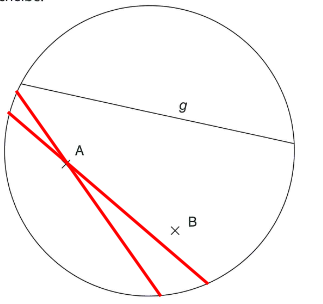
\includegraphics[width=0.8\textwidth]{Kreisscheibe.png}     
    \caption{24}     
    \label{fig:24} 
\end{figure}
\subsubsection*{Begründe, weshalb bei dieser Geometrie das Parallelenaxiom nicht erfüllt ist.}
Weil es z.B. zum Punkt A und der Gerade g zwei Geraden gibt, die keinen gemeinsamen Punkt mit g haben, wie oben eingezeichnet.
\subsubsection*{Sind eigentlich die ersten drei Axiome erfüllt?}
1) Jeder Gerade enthält mindestens zwei Punkte.\\
Ja, da jede Sehne durch das Innere des Kreises gehen muss und zwei verschiedene Randpunkte hat die sie verbindet, gibt es sogar unendlich viele Punkte welche zwischen den Randpunkten der Sehne liegen und somit im inneren des Kreisesund auf der Sehne liegen.
2) Zu zwei verschiedenen Punkten gibt es stets genau eine Gerade, auf der die beiden Punkte liegen.\\
Ja, denn für alle Punktepaare (innerhalb des Kreises) gibt es eine eindeutige euklidische Gerade durch diese beiden Punkte, die Strecke welche die Schnittpunkte der Geraden mit dem Kreis verbindet ist dann die eindeutige Gerade auf der Kreisscheibe.\\
3) Es gibt mindestens drei Punkte, die nicht alle auf derselben Geraden liegen.\\
Wenn man zwei Punkte hat, die auf einer Sehne liegen, kann man sich trivialer weiße einen Punkte nehmen welche nicht auf der Sehne liegt und im inneren des Kreises ist.

\newpage
\begin{figure}[htbp]     
    \centering             
    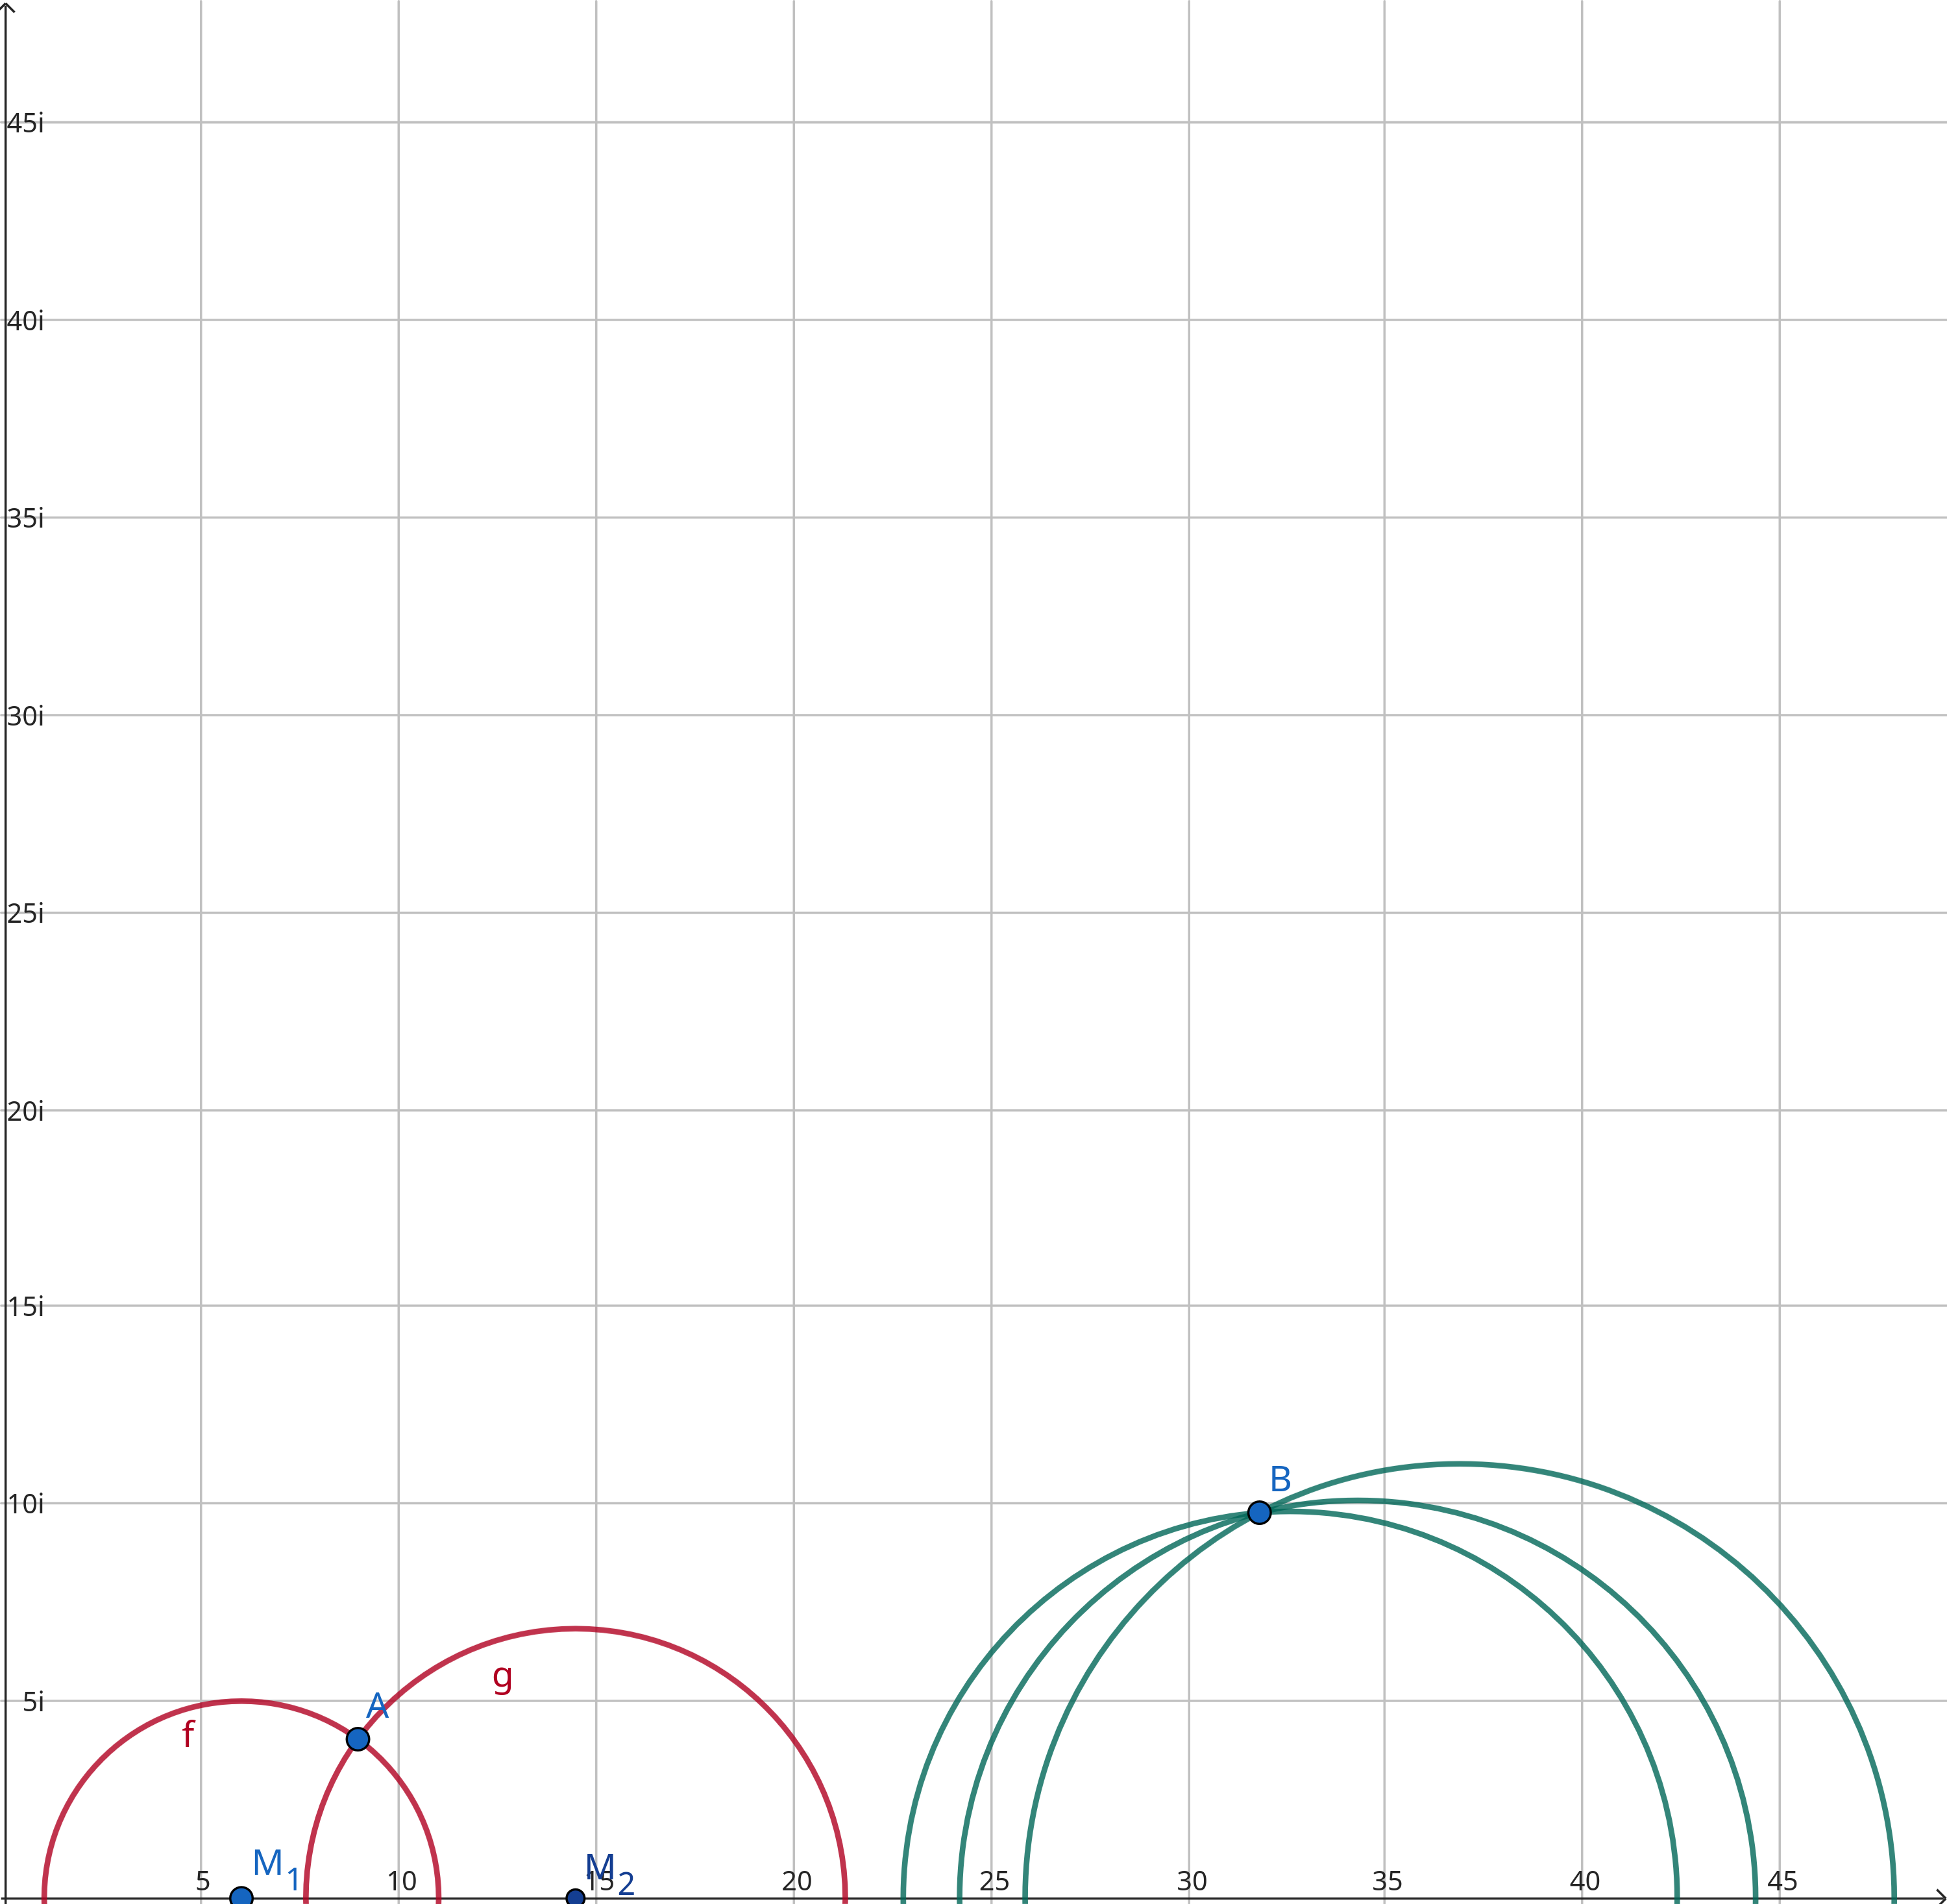
\includegraphics[width=0.8\textwidth]{Hyperbolisch.png}     
    \caption{24}     
    \label{fig:24} 
\end{figure}
\subsubsection*{Prüfe nach, ob die ersten drei Axiome für diese Geometrie erfüllt werden.}
1) Jeder Gerade enthält mindestens zwei Punkte.\\
Ein nicht-entarteter Halbkreis besteht definitionsgemäß aus unendlich vielen Punkten, da jeder Wert xx im Intervall zwischen den Schnittpunkten des Halbkreises mit der xx-Achse einem Punkt auf dem Halbkreis entspricht. Da die reellen Zahlen im Intervall dicht liegen, gibt es zwischen beliebigen zwei Punkten auf dem Halbkreis immer noch weitere Punkte. Somit enthält jede solche „Gerade“ nicht nur mindestens zwei, sondern sogar unendlich viele Punkte.\\
2) Zu zwei verschiedenen Punkten gibt es stets genau eine Gerade, auf der die beiden Punkte liegen.\\
Ja, denn man kann die eindeutige Strecke zwischen den Punkten bestimmen, dazu die eindeutige Mittelsenkrechte und dann den eindeutigen Schnittpunkt mit der $x$-Achse, welcher der Mittelpunkt des Halbkreises sein muss. Dieser ist somit auch eindeutig.\\  
3) Es gibt mindestens drei Punkte, die nicht alle auf derselben Geraden liegen.\\
Nimmt man die Punkte (1, 1), (2, 1) und (3, 1) dann gibt es einen eindeutigen Halbkreis $hk_1$ durch (1, 1) und (2, 1) und es gibt einen eindeutigen Halbkreis $hk_2$ durch (2, 1) und (3, 1). Diese Halbkreise sind offensichtlich verschieden und (3, 1) liegt nicht auf $hk_1$ und (1, 1) liegt nicht auf $hk_2$.
\subsubsection*{Trifft das auch auf das Parallelenaxiom zu?}
Nein, denn es gibt zu $g$ unendlich viele Geraden die durch einen Punkt A gehen welcher nicht auf $g$ liegt und keinen Schnittpunkt mit $g$ haben. (Oben in grün eingezeichnet.)
\subsubsection*{Wie findest du zu zwei "Punkten" die passende "Gerade", die durch diese beiden Punkte geht? Begründe, dass es nur eine solche geben kann.}
Man kann die eindeutige Strecke zwischen den Punkten bestimmen, dazu die eindeutige Mittelsenkrechte und dann den eindeutigen Schnittpunkt mit der $x$-Achse, welcher der Mittelpunkt des Halbkreises sein muss. Dieser ist somit auch eindeutig.\\

\subsection*{(ii) Erklären Sie, was mit folgendem Satz gemeint ist: „Axiomensysteme werden durch Modelle interpretiert“.}
\subsubsection*{(a) In Bezug auf das Schülerarbeitsblatt „Lass Krummes mal Gerade sein“.}
Das Arbeitsblatt beschäftigt sich damit, wie man geometrische Grundbegriffe (wie „Punkt“ und „Gerade“) und deren Beziehungen durch Axiome festlegt, ohne sie direkt zu definieren.\\ 
\textbf{Beispiel:}\\ 
Das Axiom „Durch zwei verschiedene Punkte geht genau eine Gerade“ beschreibt eine Beziehung, aber nicht, was „Punkt“ oder „Gerade“ konkret sind.\\ 
\textbf{Interpretation durch Modelle:}\\ 
Ein Modell könnte zum Beispiel die klassische euklidische Ebene sein, in der Punkte gewöhnliche Punkte auf dem Papier und Geraden die üblichen Linien sind. Ein anderes Modell könnte die „Geraden“ als Kreise oder andere Objekte interpretieren, solange die Axiome erfüllt bleiben.\\ 
\textbf{Im Kontext des Arbeitsblatts:}\\ 
Das Arbeitsblatt zeigt, dass die Axiome unabhängig von einer bestimmten Vorstellung gelten. Erst durch die Wahl eines Modells (z.B. das Papier mit Punkten und Linien) wird festgelegt, was die abstrakten Begriffe konkret bedeuten.\\ 
\textbf{Fazit:}\\ 
Die Schüler lernen, dass die Axiome ein abstraktes Gerüst liefern und erst durch Modelle anschaulich oder praktisch werden.

\newpage
\subsubsection*{(b) In Bezug auf die Vorlesung „Elementargeometrie“.}
Ein Axiomensystem ist eine Sammlung von Grundannahmen (Axiomen), die als Ausgangspunkt für ein mathematisches Theoriesystem dienen. \\ 
Diese Axiome sind abstrakt formuliert und verwenden sogenannte \emph{unbestimmte Begriffe}, deren genaue Bedeutung zunächst offen bleibt. \\ 
Ein \textbf{Modell} eines Axiomensystems ist eine konkrete mathematische Struktur, in der \\ 
\hspace*{1em} -- die unbestimmten Begriffe durch bestimmte mathematische Objekte ersetzt werden, \\ 
\hspace*{1em} -- und die Axiome als wahre Aussagen gelten. \\ Der Satz „Axiomensysteme werden durch Modelle interpretiert“ bedeutet: \\ 
\hspace*{1em} -- Die abstrakten Axiome bekommen erst durch die Wahl eines Modells eine konkrete Bedeutung. \\ 
\hspace*{1em} -- Unterschiedliche Modelle können denselben Axiomen verschiedene Inhalte geben. \\ 
In der Geometrie werden die Grundbegriffe wie „Punkt“, „Gerade“ und „Ebene“ durch Axiome (z.B. die euklidischen Axiome) in Beziehung gesetzt, ohne sie anschaulich zu definieren. \\ 
Ein \textbf{Modell} in der Geometrie bedeutet: \\ 
\hspace*{1em} -- Man ordnet den Begriffen „Punkt“, „Gerade“ usw. konkrete mathematische Objekte zu (z.B. Punkte und Geraden in der Ebene, Kreise, Kugeln usw.). \\ 
\hspace*{1em} -- Das Modell ist genau dann ein Modell des Axiomensystems, wenn alle Axiome in dieser Zuordnung erfüllt sind. \\ 
\textbf{Beispiele:} \\ 
\hspace*{1em} -- In der klassischen euklidischen Geometrie sind „Punkte“ die Elemente von $\mathbb{R}^2$ und „Geraden“ die üblichen Geraden. \\ 
\hspace*{1em} -- Auch exotische Modelle sind möglich, z.B. in der hyperbolischen Geometrie \\ 
\textbf{Fazit für die Geometrie:} \\ 
Die Axiome definieren ein Regelwerk, das durch verschiedene Modelle mit Leben gefüllt werden kann. \\ 
Erst durch das Modell wird festgelegt, was „Punkt“ und „Gerade“ konkret bedeuten. \\ 
Die Geometrie ist also nicht an eine bestimmte Anschauung gebunden, sondern an die Struktur der Axiome und deren Modelle. \\ 
\end{document}
